% Embedded Systems lab report -- compile with pdflatex (twice, for the ToC)
\documentclass[11pt,a4paper]{article}

\usepackage[margin=2.5cm]{geometry}
\usepackage{lmodern}      % scalable Type1 fonts for T1; without this,
\usepackage[T1]{fontenc}  % MiKTeX builds slow, fuzzy METAFONT bitmaps
\usepackage[utf8]{inputenc}
\usepackage{amsmath}
\usepackage{graphicx}
\usepackage{float}
\usepackage{array}
\usepackage{booktabs}
\usepackage{xcolor}
\usepackage{listings}
\usepackage[hidelinks]{hyperref}

% --- C code listing style -------------------------------------------------
\definecolor{codegray}{gray}{0.96}
\definecolor{codegreen}{rgb}{0.0,0.5,0.0}
\definecolor{codeblue}{rgb}{0.0,0.0,0.6}

\lstdefinestyle{cstyle}{
  language=C,
  backgroundcolor=\color{codegray},
  basicstyle=\ttfamily\footnotesize,
  keywordstyle=\color{codeblue}\bfseries,
  commentstyle=\color{codegreen}\itshape,
  stringstyle=\color{red!70!black},
  numbers=left,
  numberstyle=\tiny\color{gray},
  numbersep=8pt,
  breaklines=true,
  frame=single,
  framerule=0pt,
  showstringspaces=false,
  tabsize=4,
  captionpos=b,
}
\lstset{style=cstyle}

\newcommand{\us}{\,\text{\textmu s}}
\newcommand{\dg}{\text{\textdegree}}
\setlength{\emergencystretch}{2em}

% --- Title ----------------------------------------------------------------
\newcommand{\studentid}{R12942157}

\title{Embedded Systems Laboratory Report\\
       \large PWM Generation and Input Capture with STM32 Timers\\
       \normalsize Basic Problem and Option Problem 1(a)}
\author{YU-CHEN, CHU\\
        \normalsize Student ID: \studentid}
\date{\today\\[2ex]
      \normalsize Source code:
      \url{https://github.com/oldpig123/embedded_system/tree/master/lab5}}

\begin{document}
\maketitle
\tableofcontents
\newpage

% =========================================================================
\section{Introduction}

Pulse-width modulation (PWM) puts a value into the width of a pulse that
repeats at a fixed rate. The ratio of the high time to the period is the
\emph{duty cycle}. LED dimmers, motor drivers, switching power supplies and
hobby servos all use PWM.

For the basic problem I chose the hobby servo. A servo reads a 50\,Hz pulse
train and turns its shaft to the angle that the pulse width sets. I did not
have a servo. The assignment asks for the waveform on a logic analyzer, so the
logic analyzer takes the place of the servo in this lab.

Option problem~1 has two parts. Part~(b), complementary PWM with dead time,
needs a Nucleo board from the TA, because the IoT board has too few free timer
pins. I did part~(a), input capture. A second timer on the same board measures
the servo signal and converts the pulse width back into an angle. The control
circuit inside a real servo does the same job.

% =========================================================================
\section{Environment}

\begin{table}[h]
\centering
\caption{Hardware and software.}
\begin{tabular}{@{}lp{11.5cm}@{}}
\toprule
Board            & B-L475E-IOT01A (STM32L475VG, Cortex-M4, 80\,MHz) \\
Configuration    & STM32CubeMX 6.18.1, STM32Cube FW\_L4 V1.18.2 (HAL) \\
Build            & CMake, Ninja, \texttt{arm-none-eabi-gcc} 14.3.1, VS Code with the STM32Cube extension \\
Logic analyzer   & Zeroplus LAP-C(16128): 16 channels, 128\,Kbit per channel, software V3.14.14 \\
Serial output    & USART1 to the ST-LINK virtual COM port, 115200 baud, 8N1, VS Code Serial Monitor \\
\bottomrule
\end{tabular}
\end{table}

The system clock comes from the 4\,MHz MSI oscillator through the PLL
($\times 40$, $\div 2$), which gives 80\,MHz. The LSE crystal calibrates the
MSI continuously (MSI PLL mode). The APB1 bus has no divider, so TIM2 and TIM3
receive 80\,MHz before their prescalers.

\begin{table}[h]
\centering
\caption{Connections. CN1 and CN3 are the Arduino headers (UM2153, Table~4).}
\begin{tabular}{@{}lll@{}}
\toprule
From & To & Signal \\
\midrule
Logic analyzer GND & CN1 pin 7 & Ground \\
Logic analyzer A0  & CN1 pin 2 (D9) & PA15, TIM2\_CH1 output \\
Jumper wire        & CN1 pin 2 (D9) to CN3 pin 6 (D5) & PA15 to PB4, TIM3\_CH1 input \\
\bottomrule
\end{tabular}
\end{table}

The board-default CubeMX setup makes PB4 a GPIO output. I reassigned PB4 to
TIM3\_CH1 and flashed that program before I connected the jumper wire.
Otherwise two outputs drive the same wire.

% =========================================================================
\section{Timers and PWM}

\subsection{Formulas}

The timer counter advances once for every $\text{PSC}+1$ cycles of the timer
clock $f_\text{CK}$. It counts from 0 to ARR and then starts again at 0. So
one period has $\text{ARR}+1$ ticks:
\begin{equation}
  f_\text{tick} = \frac{f_\text{CK}}{\text{PSC}+1}, \qquad
  T_\text{PWM}  = \frac{\text{ARR}+1}{f_\text{tick}}, \qquad
  D = \frac{\text{CCR}}{\text{ARR}+1}.
\end{equation}
In PWM mode~1 the counter counts up. The output is high while
$\text{CNT} < \text{CCR}$ and low for the rest of the period. So the high time
is exactly CCR ticks.

Two details in the lecture notes need care:
\begin{itemize}
  \item Slide~6 gives the duty cycle as CCR/ARR. The exact value is
        CCR/(ARR$+1$).
  \item The bullets on slide~22 give ``Pulse (CCR) 2500000-1''. The code on
        the same slide uses \texttt{249999}, so the bullet is a typo. The
        ``$-1$'' belongs to PSC and ARR only. CCR\,=\,250000 gives exactly
        25\,\%.
\end{itemize}

\subsection{Lecture example}

As a first check of the tools, I built the example from the lecture:
TIM2\_CH1 on PA15, PSC\,=\,15, ARR\,=\,999999, CCR\,=\,249999. TIM2 is a
32-bit timer, so this ARR is valid. The tick is $80\,\text{MHz}/16 =
5\,\text{MHz}$, the period is $10^6 / 5\,\text{MHz} = 200$\,ms (5\,Hz), and the
high time is 50\,ms.

The capture window of the logic analyzer is the memory depth divided by the
sample rate. At 1\,kHz with 2K samples, the window is 2.048\,s, which holds
about 10 periods. Figure~\ref{fig:la5hz} shows the result. The marker T is on a
rising edge, A on the next falling edge and B on the next rising edge.
A$-$T\,=\,50 samples (50\,ms high) and B$-$T\,=\,200 samples (200\,ms period)
agree with the calculation.

\begin{figure}[h]
\centering
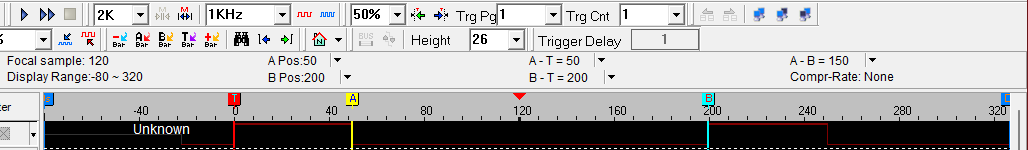
\includegraphics[width=\textwidth]{figures/la_5hz_25pct.png}
\caption{Lecture example at 1\,kHz sampling: A$-$T\,=\,50\,ms high time,
         B$-$T\,=\,200\,ms period, so 5\,Hz and 25\,\% duty.}
\label{fig:la5hz}
\end{figure}

% =========================================================================
\section{Basic Problem: Servo Control Signal}

\subsection{The application}

A hobby servo expects one pulse every 20\,ms (50\,Hz). The pulse width sets the
angle. A common convention maps 1.0\,ms to 0\dg, 1.5\,ms to 90\dg{} and
2.0\,ms to 180\dg. The exact limits differ between servo models. The program
steps the pulse width through 1.0, 1.5 and 2.0\,ms, with 1\,s at each step, as
a controller does when it moves a servo between three positions.

\subsection{Timer design}

I chose a tick of 1\us. Then ARR$+1$ and CCR are in microseconds directly.
TIM3 uses the same tick in the option problem, so both timers count in the
same unit.

\begin{table}[h]
\centering
\caption{TIM2 settings for the lecture example and for the servo signal.}
\begin{tabular}{@{}lll@{}}
\toprule
 & Lecture example & Servo signal \\
\midrule
PSC          & 15 (5\,MHz tick)        & $80\,\text{MHz}/1\,\text{MHz} - 1 = 79$ (1\us{} tick) \\
ARR          & 999999 (200\,ms)        & $20\,\text{ms}/1\us - 1 = 19999$ (20\,ms) \\
CCR (Pulse)  & 249999 (50\,ms)         & 1000, 1500, 2000 (1.0, 1.5, 2.0\,ms) \\
Mode         & PWM mode 1, polarity high & PWM mode 1, polarity high \\
\bottomrule
\end{tabular}
\end{table}

One tick of 1\us{} is $180\dg / 1000\us = 0.18\dg$ of servo angle. This is
the resolution of the signal.

\subsection{Implementation}

CubeMX generates \texttt{MX\_TIM2\_Init()} with the values above. The user
code starts the PWM output once. The main loop then changes CCR1 with
\texttt{\_\_HAL\_TIM\_SET\_COMPARE()} and waits 1\,s at each step.

\begin{lstlisting}[caption={Starting the PWM and stepping the pulse width (\texttt{main.c}, user code blocks 2 and 3). The \texttt{print\_measurement()} calls belong to the option problem.}]
/* USER CODE BEGIN 2 */
HAL_TIM_PWM_Start(&htim2, TIM_CHANNEL_1);

/* USER CODE BEGIN 3 */
__HAL_TIM_SET_COMPARE(&htim2, TIM_CHANNEL_1, 1000);
HAL_Delay(1000);
print_measurement(period, pulse_width);
__HAL_TIM_SET_COMPARE(&htim2, TIM_CHANNEL_1, 1500);
HAL_Delay(1000);
print_measurement(period, pulse_width);
__HAL_TIM_SET_COMPARE(&htim2, TIM_CHANNEL_1, 2000);
HAL_Delay(1000);
print_measurement(period, pulse_width);
\end{lstlisting}

\subsection{Results}

I sampled at 10\,kHz with 2K samples. One sample is 0.1\,ms, and the window
is 205\,ms, which holds about 10 periods. I took one capture at each step. The markers are placed as in Figure~\ref{fig:la5hz}, so
A$-$T is the high time and B$-$T is the period.

\begin{table}[h]
\centering
\caption{Expected and measured values at 10\,kHz sampling (1 sample = 0.1\,ms).}
\begin{tabular}{@{}cccccc@{}}
\toprule
CCR & Angle & High time & A$-$T (samples) & Period & B$-$T (samples) \\
\midrule
1000 & 0\dg   & 1.0\,ms & 10 & 20\,ms & 200 \\
1500 & 90\dg  & 1.5\,ms & 15 & 20\,ms & 200 \\
2000 & 180\dg & 2.0\,ms & 20 & 20\,ms & 200 \\
\bottomrule
\end{tabular}
\end{table}

All values agree with the design. The resolution of this measurement is
$\pm 1$ sample ($\pm 0.1$\,ms).

\begin{figure}[h]
\centering
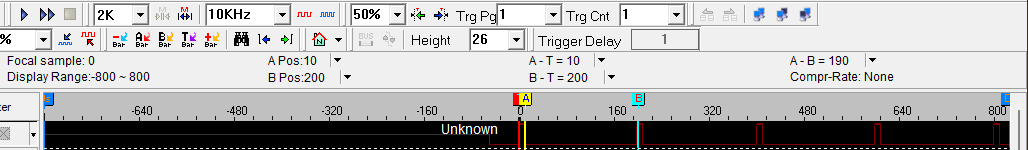
\includegraphics[width=\textwidth]{figures/la_servo_1000us.png}\\[0.3ex]
{\small (a) CCR\,=\,1000: A$-$T\,=\,10, B$-$T\,=\,200}\\[1.5ex]
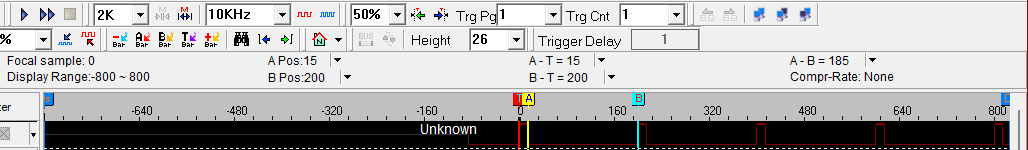
\includegraphics[width=\textwidth]{figures/la_servo_1500us.png}\\[0.3ex]
{\small (b) CCR\,=\,1500: A$-$T\,=\,15, B$-$T\,=\,200}\\[1.5ex]
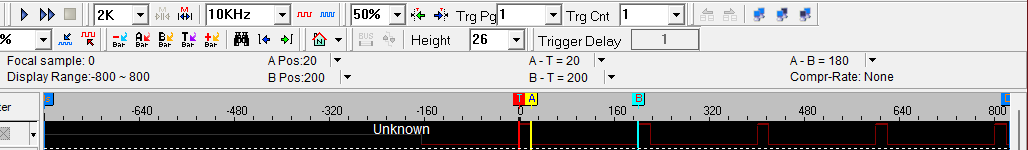
\includegraphics[width=\textwidth]{figures/la_servo_2000us.png}\\[0.3ex]
{\small (c) CCR\,=\,2000: A$-$T\,=\,20, B$-$T\,=\,200}
\caption{The servo signal at the three steps, 10\,kHz sampling.}
\label{fig:servo}
\end{figure}

\subsection{Changing CCR while the timer runs}
\label{sec:preload}

The main loop writes CCR1 at a random time in the period. Figure~\ref{fig:step}
shows a capture that contains a step from 2000 to 1000. Pulses of 20 samples
come first, then pulses of 10 samples. The period stays 200 samples, and no pulse
has a wrong width.

\begin{figure}[h]
\centering
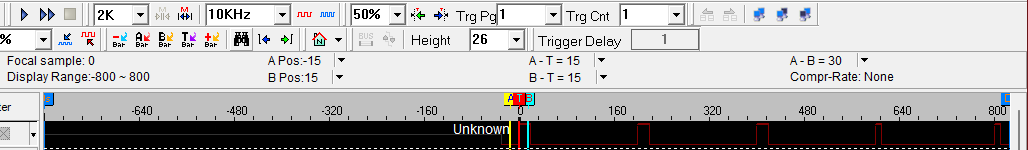
\includegraphics[width=\textwidth]{figures/la_servo_step.png}
\caption{A step from CCR\,=\,2000 to 1000 inside one capture. The markers in
         this capture are not on edges, so their read-outs have no meaning.}
\label{fig:step}
\end{figure}

The reason is the \emph{preload} of the compare register.
\texttt{HAL\_TIM\_PWM\_ConfigChannel()} sets the OC1PE bit. With OC1PE set, a
write to CCR1 goes into a preload register. The timer copies this value into
the active register at the next update event, which is the start of a period.
Without preload, the new value acts at once. A write of 1000 while the counter
is at 1500 ends the pulse at 1.5\,ms, which is neither the old nor the new
width. A write of 2000 while the counter is at 1200 makes a second pulse in the
same period. A real servo reads such a pulse as a wrong angle.

% =========================================================================
\section{Option Problem 1(a): Input Capture}

\subsection{Setup}

TIM3 is a 16-bit general-purpose timer. Its channel~1 input is PB4, which is
D5 on the Arduino header. The jumper wire from D9 to D5 brings the TIM2 output
to TIM3. TIM3 uses PSC\,=\,79 (1\us{} tick) and ARR\,=\,65535, the maximum.
USART1 sends the result to the PC once per second, after each step of the
sweep.

I used two methods. Method~A follows the hint article from the ST community
(\emph{How to use the input capture feature}). Method~B uses the PWM input mode
of the reference manual (RM0351, section~31.3.6).

\subsection{Method A: period from two captures}

Channel~1 is in input capture mode: direct input, rising edge, no filter, with
the TIM3 interrupt on. At each rising edge, the timer copies CNT into CCR1 and
HAL calls \texttt{HAL\_TIM\_IC\_CaptureCallback()}. The callback subtracts the
previous capture from the current one.

\begin{lstlisting}[caption={Method A callback. The final source contains only the Method B version (Listing~\ref{lst:methodb}).}]
void HAL_TIM_IC_CaptureCallback(TIM_HandleTypeDef *htim)
{
    if (htim->Instance == TIM3 && htim->Channel == HAL_TIM_ACTIVE_CHANNEL_1)
    {
        static uint16_t previous_capture = 0;
        uint16_t current_capture = HAL_TIM_ReadCapturedValue(htim, TIM_CHANNEL_1);
        period = current_capture - previous_capture;
        previous_capture = current_capture;
    }
}
\end{lstlisting}

The counter wraps from 65535 to 0, but the subtraction still gives the right
result. C converts both operands to \texttt{int}, so for example
$3000 - 60000 = -57000$. The assignment to the \texttt{uint16\_t} variable
reduces this modulo 65536 to 8536, which is the correct number of ticks. This
works only while one period is shorter than 65536 ticks (65.5\,ms). Then at
most one wrap occurs between two captures.

The first result is wrong, because \texttt{previous\_capture} starts at 0. The
callback runs 50 times per second and the program prints once per second, so a
correct value replaces the wrong one before the first print.
Figure~\ref{fig:parta} shows the output: 20000\us{} on every line.

\begin{figure}[h]
\centering
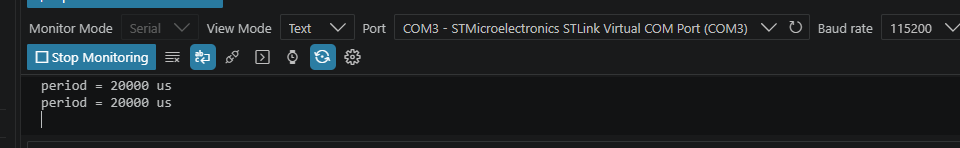
\includegraphics[width=0.85\textwidth]{figures/uart_part_a.png}
\caption{Method A output on the serial monitor.}
\label{fig:parta}
\end{figure}

\subsection{Method B: PWM input mode}

Method~A gives only the period. The servo information is in the pulse width,
so the falling edge is necessary too. In PWM input mode, two capture channels
read the same input pin (TI1). The reference manual gives the procedure:

\begin{enumerate}
  \item Channel~1 reads TI1 directly and captures on the rising edge.
  \item Channel~2 reads TI1 indirectly and captures on the falling edge.
  \item The trigger input is TI1FP1, and the slave mode controller is in
        \emph{reset} mode. Each rising edge resets the counter to 0.
\end{enumerate}

So CCR1 holds the period and CCR2 holds the high time. The program needs no
subtraction and no overflow handling.

CubeMX offers a shortcut for this mode (Combined Channels, \emph{PWM Input on
CH1}), but it was not available in this project. I set the two channels one by
one instead, which gives the same register settings. CubeMX uses one settings
structure for both channels and writes only the fields that change. Thus the
falling edge for channel~2 must be set in CubeMX explicitly. Otherwise
channel~2 captures on the rising edge too.

\begin{lstlisting}[caption={Generated TIM3 configuration (\texttt{MX\_TIM3\_Init()}, error checks removed).}]
sSlaveConfig.SlaveMode = TIM_SLAVEMODE_RESET;
sSlaveConfig.InputTrigger = TIM_TS_TI1FP1;
sSlaveConfig.TriggerPolarity = TIM_INPUTCHANNELPOLARITY_RISING;
sSlaveConfig.TriggerFilter = 0;
HAL_TIM_SlaveConfigSynchro(&htim3, &sSlaveConfig);

sConfigIC.ICPolarity = TIM_INPUTCHANNELPOLARITY_RISING;
sConfigIC.ICSelection = TIM_ICSELECTION_DIRECTTI;
sConfigIC.ICPrescaler = TIM_ICPSC_DIV1;
sConfigIC.ICFilter = 0;
HAL_TIM_IC_ConfigChannel(&htim3, &sConfigIC, TIM_CHANNEL_1);

sConfigIC.ICPolarity = TIM_INPUTCHANNELPOLARITY_FALLING;
sConfigIC.ICSelection = TIM_ICSELECTION_INDIRECTTI;
HAL_TIM_IC_ConfigChannel(&htim3, &sConfigIC, TIM_CHANNEL_2);
\end{lstlisting}

Only channel~1 has an interrupt. At a rising edge, CCR1 holds the length of the
period that just ended. CCR2 holds the high time of the same period, because
its falling edge came before this rising edge. So the two values always belong
together.

\begin{lstlisting}[label={lst:methodb},caption={Method B user code (\texttt{main.c}, user code blocks PV, 0, 2 and 4).}]
/* USER CODE BEGIN PV */
volatile uint16_t period = 0; // Variable to store the measured period
volatile uint16_t pulse_width = 0; // Variable to store the measured pulse width

/* USER CODE BEGIN 0 */
static void print_measurement(uint16_t period, uint16_t pulse_width) {
    char buffer[80];
    snprintf(buffer, sizeof(buffer), "period = %u us, width = %u us, angle = %d dg\r\n", period, pulse_width, (int)((pulse_width - 1000) * 180 / 1000));
    HAL_UART_Transmit(&huart1, (uint8_t*)buffer, strlen(buffer), HAL_MAX_DELAY);
}

/* USER CODE BEGIN 2 */
HAL_TIM_PWM_Start(&htim2, TIM_CHANNEL_1);
HAL_TIM_IC_Start(&htim3, TIM_CHANNEL_2);
HAL_TIM_IC_Start_IT(&htim3, TIM_CHANNEL_1);

/* USER CODE BEGIN 4 */
void HAL_TIM_IC_CaptureCallback(TIM_HandleTypeDef *htim)
{
    if (htim->Instance == TIM3 && htim->Channel == HAL_TIM_ACTIVE_CHANNEL_1)
    {
        period = HAL_TIM_ReadCapturedValue(htim, TIM_CHANNEL_1)+1;
        pulse_width = HAL_TIM_ReadCapturedValue(htim, TIM_CHANNEL_2)+1;
    }
}
\end{lstlisting}

The angle is $(\text{width} - 1000) \times 180 / 1000$ in \texttt{int}
arithmetic. The \texttt{uint16\_t} width becomes \texttt{int} before the
subtraction, so a width below 1000 gives a negative angle and not a large
positive number.

\subsection{Results and the ``+1''}

The first version of the callback stored the register values without the
``+1''. Figure~\ref{fig:partbraw} shows its output. Every value is 1\us{} too
small: 19999 instead of 20000, and 999, 1499 and 1999 instead of 1000, 1500
and 2000.

\begin{figure}[h]
\centering
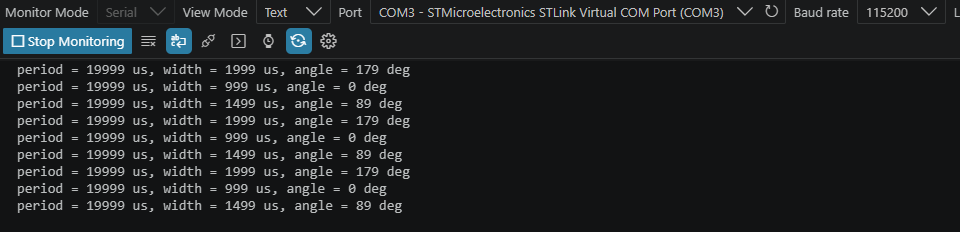
\includegraphics[width=0.85\textwidth]{figures/uart_part_b_raw.png}
\caption{Method B output before the correction. All values are one tick low.}
\label{fig:partbraw}
\end{figure}

Figure~312 of RM0351 (\emph{PWM input mode timing}) shows the same behavior.
In that figure the counter goes through 0000 to 0004, which is a period of
5 ticks, and CCR1 holds 0004. The input is high during 0000 to 0002, which is
3 ticks, and CCR2 holds 0002. The reset sets the counter to 0, so a time of
$n$ ticks shows the counter values 0 to $n-1$. The capture stores the last of
these values. Thus the true values are $\text{CCR1}+1$ and $\text{CCR2}+1$.
This is the same ``+1'' as in ARR: ARR\,=\,19999 makes 20000 ticks, and the
capture of those 20000 ticks reads 19999.

Method~A did not show this offset. Each of its two captures has the same
offset, and the subtraction removes it. Method~B measures from a counter that
starts at 0, so the offset stays.

Two effects together made the angle 1\dg{} low. The width 1999 gives
$999 \times 180 / 1000 = 179.82$, and integer division truncates this to 179.
At 0\dg{} the error did not show: 999 gives $-0.18$, and C truncates toward
zero, which gives 0. After the correction in the callback, the output is
exact (Figure~\ref{fig:partb}).

\begin{figure}[h]
\centering
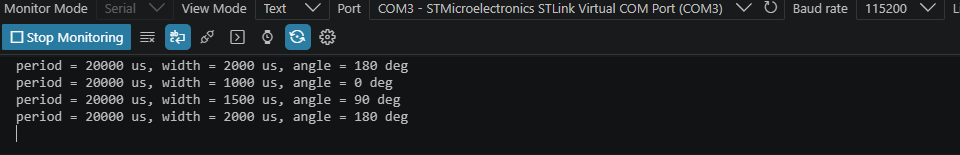
\includegraphics[width=0.85\textwidth]{figures/uart_part_b.png}
\caption{Method B output after the correction: period, width and angle for
         the steps 2000, 1000, 1500 and 2000.}
\label{fig:partb}
\end{figure}

\subsection{Discussion}

\paragraph{Method A and method B.}
Table~\ref{tab:methods} compares the two methods. Method~A works on any
capture channel and keeps the counter free. Method~B does more in hardware,
but it needs a channel pair. Only TI1FP1 and TI2FP2 connect to the slave mode
controller, so PWM input mode works only on channels~1 and~2 (RM0351, note to
Figure~312).

\begin{table}[h]
\centering
\caption{Comparison of the two capture methods.}
\label{tab:methods}
\begin{tabular}{@{}lll@{}}
\toprule
 & Method A (two captures) & Method B (PWM input mode) \\
\midrule
Measures             & Period                      & Period and high time \\
Channels             & 1 (any channel)             & 2 (channels 1 and 2 only) \\
Counter              & Runs freely, wraps          & Reset at each rising edge \\
Work in software     & Subtraction, wrap handling  & Two register reads \\
Interrupts per period & 1                          & 1 \\
Offset               & Cancels in the subtraction  & $-1$ tick, corrected with $+1$ \\
\bottomrule
\end{tabular}
\end{table}

\paragraph{Resolution and range.}
The 1\us{} tick gives a resolution of 1\us, which is 0.18\dg{} of servo
angle. The 16-bit counter limits the period to 65535\us. The 20\,ms servo
period uses about 30\,\% of this range. A slower signal needs a larger PSC,
which makes the resolution coarser, or a 32-bit timer such as TIM2 or TIM5. A
faster signal keeps 1\us{} resolution, but the relative error grows. At 10\,kHz
one tick is already 1\,\% of the period.

\paragraph{Clock source and accuracy.}
TIM2 and TIM3 use the same 80\,MHz clock. The edges of the signal are
therefore always at the same counter positions, and every line of the output
is identical. An error of the 80\,MHz clock changes both timers in the same
way, so the measurement cannot show it. The logic analyzer uses its own clock.
It agreed with the timers within its resolution of 0.1\,ms. A signal from a
different clock would show a jitter of $\pm 1$ tick, also after the ``+1''
correction.

\paragraph{Interrupt load and shared data.}
Both methods cause 50 interrupts per second. Each callback reads one or two
registers, so the CPU load is very small. The callback and the main loop share
\texttt{period} and \texttt{pulse\_width}. These variables are
\texttt{volatile}, so the compiler reads them from memory each time. The
Cortex-M4 reads and writes a 16-bit value in one instruction. Thus the main
loop never sees a value that is half old and half new. The main loop reads the
two variables at two different times. An interrupt between the two reads can
give a pair from two adjacent periods. This has no effect here, because the
print comes 1\,s after each step, when both values are stable.

\paragraph{Input filter.}
The input filter is off (\texttt{ICFilter = 0}). The signal comes from the same
board over a short wire and has no noise. A signal from a long cable or a
mechanical contact needs the digital filter, which adds a short delay to each
edge.

\paragraph{A note on the hint article.}
The article calculates the frequency as \texttt{HAL\_RCC\_GetPCLK1Freq()}
divided by the capture difference. This formula leaves out the prescaler. With
PSC\,=\,79 the result is 80 times too high. The correct formula is
$f = f_\text{CK} / ((\text{PSC}+1)\,\Delta)$. The article also has no overflow
handling, which Method~A adds.

% =========================================================================
\section{Problems Encountered}

Table~\ref{tab:problems} lists the problems in the order they occurred. The
row ``Found before flashing'' holds two problems from a code review. They
never reached the board.

\begin{table}[H]
\centering
\caption{Problems, their symptoms and causes.}
\label{tab:problems}
\footnotesize
\begin{tabular}{@{}>{\raggedright\arraybackslash}p{2.9cm}%
                  >{\raggedright\arraybackslash}p{5.0cm}%
                  >{\raggedright\arraybackslash}p{7.3cm}@{}}
\toprule
Problem & Symptom & Cause and fix \\
\midrule
Analyzer driver &
  The driver comes on a disc, and the laptop has no disc drive. &
  The Zeroplus download page has the same package (``LAP-C Standard''
  V3.14.14, Windows 7 to 11). It contains the driver and the software. \\
New project does not build in VS Code &
  \texttt{Bad CMake executable: ""}, then configure fails with
  \texttt{CMAKE\_MAKE\_PROGRAM-NOTFOUND}. &
  CubeMX does not create \texttt{.vscode/settings.json}
  (\texttt{cube-cmake}) or \texttt{.settings/} (tool versions). I copied both
  from an earlier lab. \\
Only the high time is visible &
  One 1.5\,ms pulse, then a flat line to the end of the capture. &
  ARR was still 999999. With a 1\us{} tick the period was 1\,s, longer than
  the 205\,ms window. ARR\,=\,19999 fixed it. \\
Steps hard to see &
  In a 64K capture all pulses look the same. &
  One step is 10000 samples. At a zoom that shows several steps, a 10-sample
  and a 20-sample pulse look equal. Repeated 2K captures show one step at a
  time. \\
\texttt{period = 0 us} &
  The value never changes. &
  The jumper wire was not connected, so the callback never ran. \\
Combined Channels not available &
  CubeMX shows the field in grey. &
  I set channel~1 (direct, rising) and channel~2 (indirect, falling) one by
  one, as in RM0351. \\
Found before flashing &
  Channel~2 polarity was rising. \texttt{gcc} warned
  \texttt{-Wformat-truncation}. &
  CubeMX keeps the polarity of channel~1 unless channel~2 has its own. The
  50-byte print buffer was too small for a 54-byte line. \\
Values one tick low &
  19999, 999, 1499, 1999. &
  The capture stores the last counter value, $n-1$ (RM0351, Figure~312).
  The callback adds 1. \\
\bottomrule
\end{tabular}
\end{table}

% =========================================================================
\section{Conclusion}

TIM2 generates a 50\,Hz hobby-servo signal with a 1\us{} tick. The main loop
steps the pulse width through 1.0, 1.5 and 2.0\,ms. The logic analyzer
confirms each step to its resolution of 0.1\,ms. The compare preload makes
each change take effect at the start of a period, so no pulse has a wrong
width.

For option problem~1(a), TIM3 measures the same signal. Method~A uses two
rising-edge captures and gives the period. Method~B uses the PWM input mode
and gives the period and the pulse width without any subtraction. Its
registers hold one tick less than the true time, as Figure~312 of the
reference manual shows. With the ``+1'' correction, the board reads back
20000\us, 1000/1500/2000\us{} and 0/90/180\dg{} exactly.

The main lesson is the ``+1'' itself. It occurs in PSC, in ARR and in the
capture registers. Each case comes from the same fact: a counter that starts
at 0 shows $n-1$ after $n$ ticks.

\end{document}
